\documentclass[HCR,PP,english]{hcr_thesis}
\graphicspath{{pics/}{logos/}}

%% Options:
%% HCR: HCR Template with Prof. Lee as default
%% ITR: ITR Template with Prof. Hirche as default

%% BA: Bachelorarbeit
%% MA: Masterarbeit
%% HS: Hauptseminar
%% PP: Projektpraktikum
%% IP: Ingenieurpraxis
%% FP: Forschungspraxis
%% SeA: Semesterarbeit (MW)

%% english
%% german
%%% last changes: 05.04.2016 (v.gabler@tum.de)

%_________MACROS_________ (optional and customizable - see output)
%% include packages for your work in here
\usepackage[colorinlistoftodos]{todonotes}        % for handling TODOs
\usepackage{setspace}
\usepackage{acronym}
\usepackage{diagbox}
\usepackage{romannum}

% using the todonotes package in some nice ways (see packages.tex)
\newcommand{\add}[2][]{\todo[color=blue!40,#1]{#2}{}}
\newcommand\optional[2][]{\todo[inline, color=cyan!40, caption={2do},
	#1]{\begin{minipage}{\textwidth-4pt}#2\end{minipage}}{}}

% math macros
\newcommand{\set}[1]{\boldsymbol{#1}}
\renewcommand{\vec}[1]{\mathbf{#1}}


%_______Start_Document______________________________________
\begin{document}

%%%%%%%%%%%%%%%%%%%%%%%%%%%%%%%%%%%%%%%%%%%%%%%%%%%%%%%%%%%%%%%
%%%%%%%%%%%%%%%%%%% title page %%%%%%%%%%%%%%%%%%%%%%%%%%%%%%%%
%%%%%%%%%%%%%%%%%%%%%%%%%%%%%%%%%%%%%%%%%%%%%%%%%%%%%%%%%%%%%%%
%% for an english theis. The title:
\title{Training an object autoencoder using synthetic data}
%% Für deutsche Arbeiten: Deutscher Titel:
% \title{Die Antwort auf Alles und Mehr - Ein Trauerspiel in 4 Akten}
% and English translation
% \titletranslation{Random Thesis With Epic \\ and Ground Breaking Results}
% data about YOU!:
\student{Weiqi Luo} 			%% your name
\yearofbirth{13.02.1995}	%% date of birth
\city{80937 Munich}								%		"
\phone{015757297878}			%% your telephone-no.
\street{Felsennelkenanger 7}	
%% if more students are involved (e.g. PP)
%--the following parted is not tested ---
% please report bugs to v.gabler@tum.de
%\studenttwo{Zweiter Student}
%\studtitletwo{}
%\studentthree{}
%\studtitlethree{}
%\studentfour{}
%\studtitlefour{}
%-----------------------------------------
\supervisor{M.Sc. Shile Li}			%% your supervisor
\start{23.10.2019}				%% start date
\finalrep{27.01.2020}						%% final presentation / date

\maketitle
% check for colors! IF there is a color besides black on your title, you just messed it up!
%%%%%%%%%%%%%%%%%%%%%%%%%%%%%%%%%%%%%%%%%%%%%%%%%%%%%%%%%%%%%%%
%%%%%%%%%%%%%%%%%%%%%%%%%%%%%%%%%%%%%%%%%%%%%%%%%%%%%%%%%%%%%%%

\newpage

%%%%%%%%%%%%%%%%%%%%%%%%%%%%%%%%%%%%%%%%%%%%%%%%%%%%%%%%%%%%%%%
%%%%%%%%%%%%%%%%%%%%% abstract %%%%%%%%%%%%%%%%%%%%%%%%%%%%%%%%
%%%%%%%%%%%%%%%%%%%%%%%%%%%%%%%%%%%%%%%%%%%%%%%%%%%%%%%%%%%%%%%
\topmargin5mm
\textheight220mm
\pagenumbering{arabic}
\phantom{u}
\begin{abstract}


Recently, object pose estimation has drawn wide attention as it plays an important role in many robotic applications. In this project, I implemented a deep-learning-based object pose estimation approach proposed in \cite{sundermeyer2018implicit}, which operates on single RGB images and yields a fast and robust estimation result. 
\end{abstract}
\newpage

%%%%%%%%%%%%%%%%%%%%% Widmung %%%%%%%%%%%%%%%%%%%%%%%%%%%%%%%%%
\phantom{u}
\phantom{1}\vspace{6cm}
\begin{center}
%Hier die Widmung oder leer lassen
\end{center}


\pagestyle{fancy}

%%%%%%%%%%%%%%%%%%%Inhaltsverzeichnis%%%%%%%%%%%%%%%%%%%%%%%%%%
\tableofcontents

%%%%%%%%%%%%%%%%%%%%%%%%%%%%%%%
% ACTUAL CONTENT OF YOUR WORK %
%%%%%%%%%%%%%%%%%%%%%%%%%%%%%%%
%%%%%%%%%%%% Kapitel - externe Dateien zur Ordnung%%%%%%%%%%%%%
%_________Einleitung__________________________________
\chapter{Introduction}
\begin{figure}[H]
	\centering
	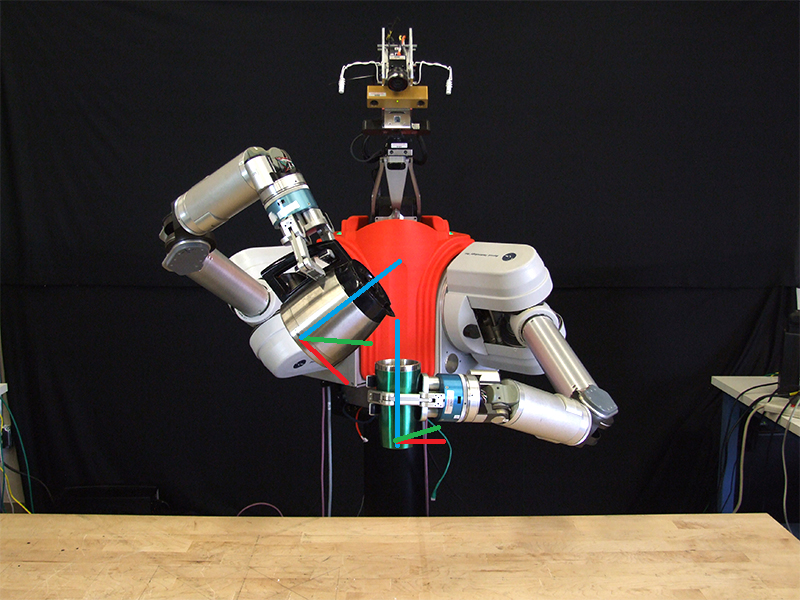
\includegraphics[width=0.75\textwidth]{intro}
	\caption[Example of object pose estimation application.]{\textbf{Example of object pose estimation application.}}
	\label{fig:intro}
\end{figure}

Fueled by the developments in robotics, autonomous driving and augmented/mixed reality, object pose estimation has become a popular research trend in computer vision. Although many encouraging achievements have emerged in recent years, a reliable and fast pose estimation still remains as an open challenge. The main deficiencies of the existing methods are (\romannumeral 1) not robust enough against object occlusions, background clutter and dynamic environment; (\romannumeral 2) often require object to have certain properties such as enough textual surface structure and asymmetric shape; (\romannumeral 3) not efficient to run in real time; (\romannumeral 4) often require a big amount of annotated training data.    
\\[8pt]
In order to conquer the above-mentioned challenges, a novel deep-learning-based approach is presented in \cite{sundermeyer2018implicit}, which operates on single RGB images and yield a fast and robust estimation in different scenarios.
\\[8pt]
In this project, I implemented the approach proposed in \cite{sundermeyer2018implicit}. I firstly generated a synthetic dataset with textured mesh model \cite{calli2015ycb}, and then trained an aotoencoder on the generated dataset. After training, I abstracted useful features from images using the autoencoder, and finally estimated the pose of the object through nearest neighbor search.

\chapter{Method}

\begin{figure}[H]
	\centering
	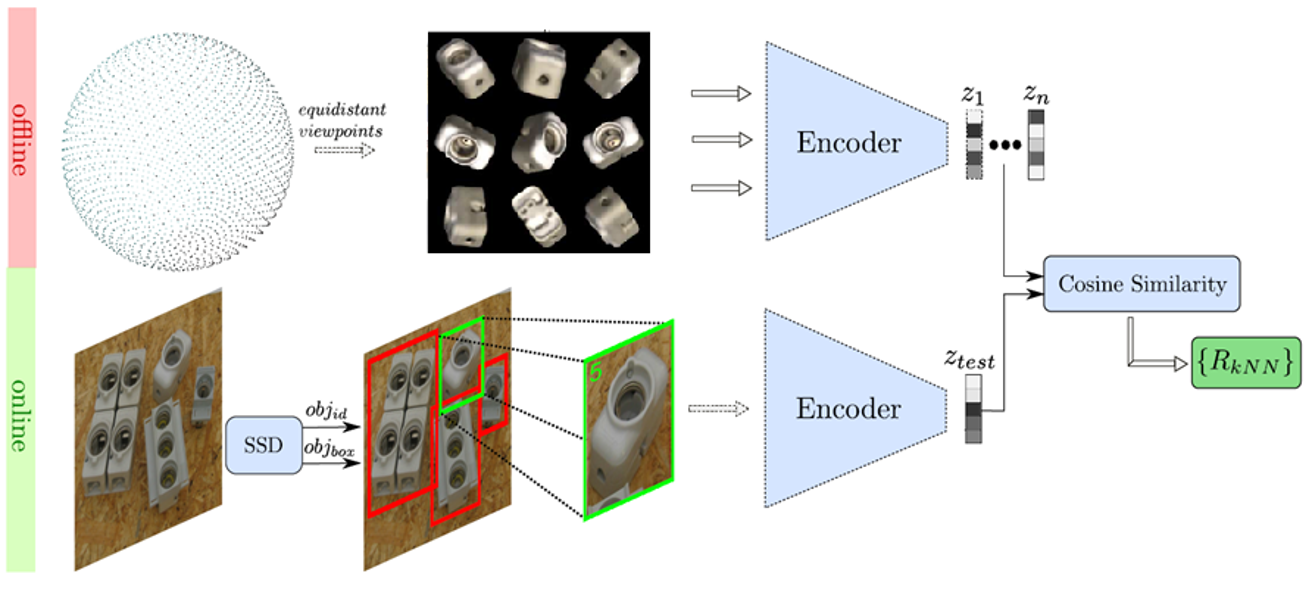
\includegraphics[width=0.9\textwidth]{structure}
	\caption[Object pose estimation pipeline]{\textbf{Object pose estimation pipeline}}
	\label{fig:structure}
\end{figure}

The main idea of this approach is to implicitly learn representations from rendered 3d model views with autoencoder, and then determine the orientation of the object employing the nearest neighbor search. On one hand, since it avoids one-to-many mappings from images to orientations, it is able to handle ambiguous poses caused by symmetric views. In another hand, it can be trained on synthetic object views in a self-supervised way and hence removes the need for a large pose-annotated dataset. Besides, by applying random augmentations on the training dataset, it is able to yield a robust estimation against occlusion and cluttered backgrounds.  \\[8pt]
The pose estimation pipeline can be divided into two parts: an offline part and an online part. In the offline part, an autoencoder is trained on the synthetic dataset, and then a codebook is created by encoding the dataset. At test time, the pose of the object is estimated using the nearest neighbor search with the highest cosine similarity from the codebook. However, due to time constraints, the object detection will not be implemented in my project.  \\[8pt]






\section{Synthetic Dataset Creation}

Since simply sampling points with permissible intervals in spherical coordinates will not result in an evenly placed points on the sphere surface, I sample viewpoints using Fibonacci Lattice as suggested in \cite{deserno2004generate}. In this sampling approach, points in the unit square $[0,\,1]$ will be first mapped to spherical coordinates with \eqref{eq:sample1}, and then be converted to euclidean coordinate using \eqref{eq:sample2}. The uniform sampling results are demonstrated in Fig. \ref{fig:uniformsample}. Fig. \ref{fig:regular} shows the regularly sampled points, while Fig. \ref{fig:random} the randomly sampled points.
  
\begin{align}
(x,\,y) \rightarrow (\theta,\, \phi) : (cos^{-1}(2x-1)-\pi /2, \, 2\pi y)
\label{eq:sample1} 
\\
(\theta,\, \phi) \rightarrow (x, \, y, \, z) : (cos \theta \, cos\phi, \, cos\theta \, sin\phi,sin \theta )
\label{eq:sample2} 
\end{align}

\begin{figure}[H]
	\centering
	\subfigure[regular sampling]{
		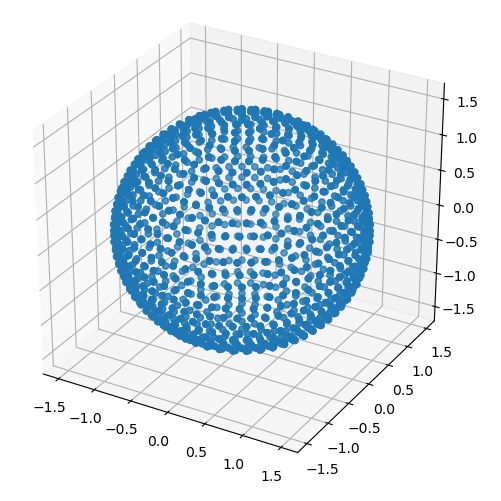
\includegraphics[width=0.4\textwidth] {uniformsampling}
		\label{fig:regular}
	}
	\qquad 
	\subfigure[random sampling]{
		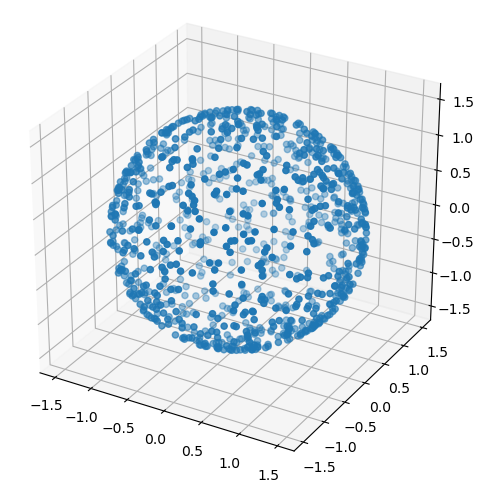
\includegraphics[width=0.4\textwidth] {randomsampling}
		\label{fig:random}
	}
	\caption[Uniform sampling of the synthetic object viewpoints]{\textbf{Uniform sampling of the synthetic object viewpoints} }
	\label{fig:uniformsample}
\end{figure}


\section{Autoencoder Training}
In order to generalize from synthetic to real data, random augmentations are applied on the rendered dataset to simulate variant real environments, and the autoencoder is trained to best reconstruct the target images from the augmented input images. The training process is illustrated in Fig. \ref{fig:autoencoder}. Fig. \ref{fig:newautoencoder} illustrates the convolutional architecture of the autoencoder used in the project, and the per-sample loss is the sum over the pixel-wise L2 distance as described in Eq. \ref{eq:loss}]. 

\begin{align}
	l_2 = \sum_{i \in \mathcal{D} } || x_{(i)}-\hat{x}_{(i)} || _2
	\label{eq:loss}
\end{align}


\begin{figure}[H]
	\centering
	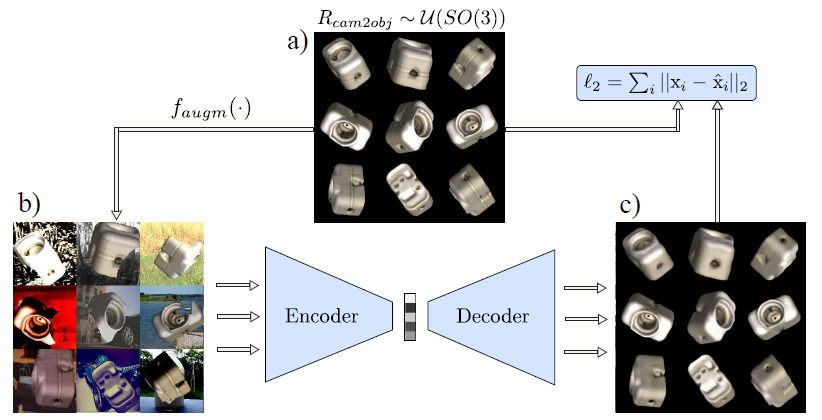
\includegraphics[width=0.8\textwidth]{autoencoder}
	\caption[Training process of the autoencoder]{\textbf{Training process of the autoencoder.} a) Reconstruction target, b) augmented input image, c) reconstructed image.}
	\label{fig:autoencoder}
\end{figure}
\begin{figure}[H]
	\centering
	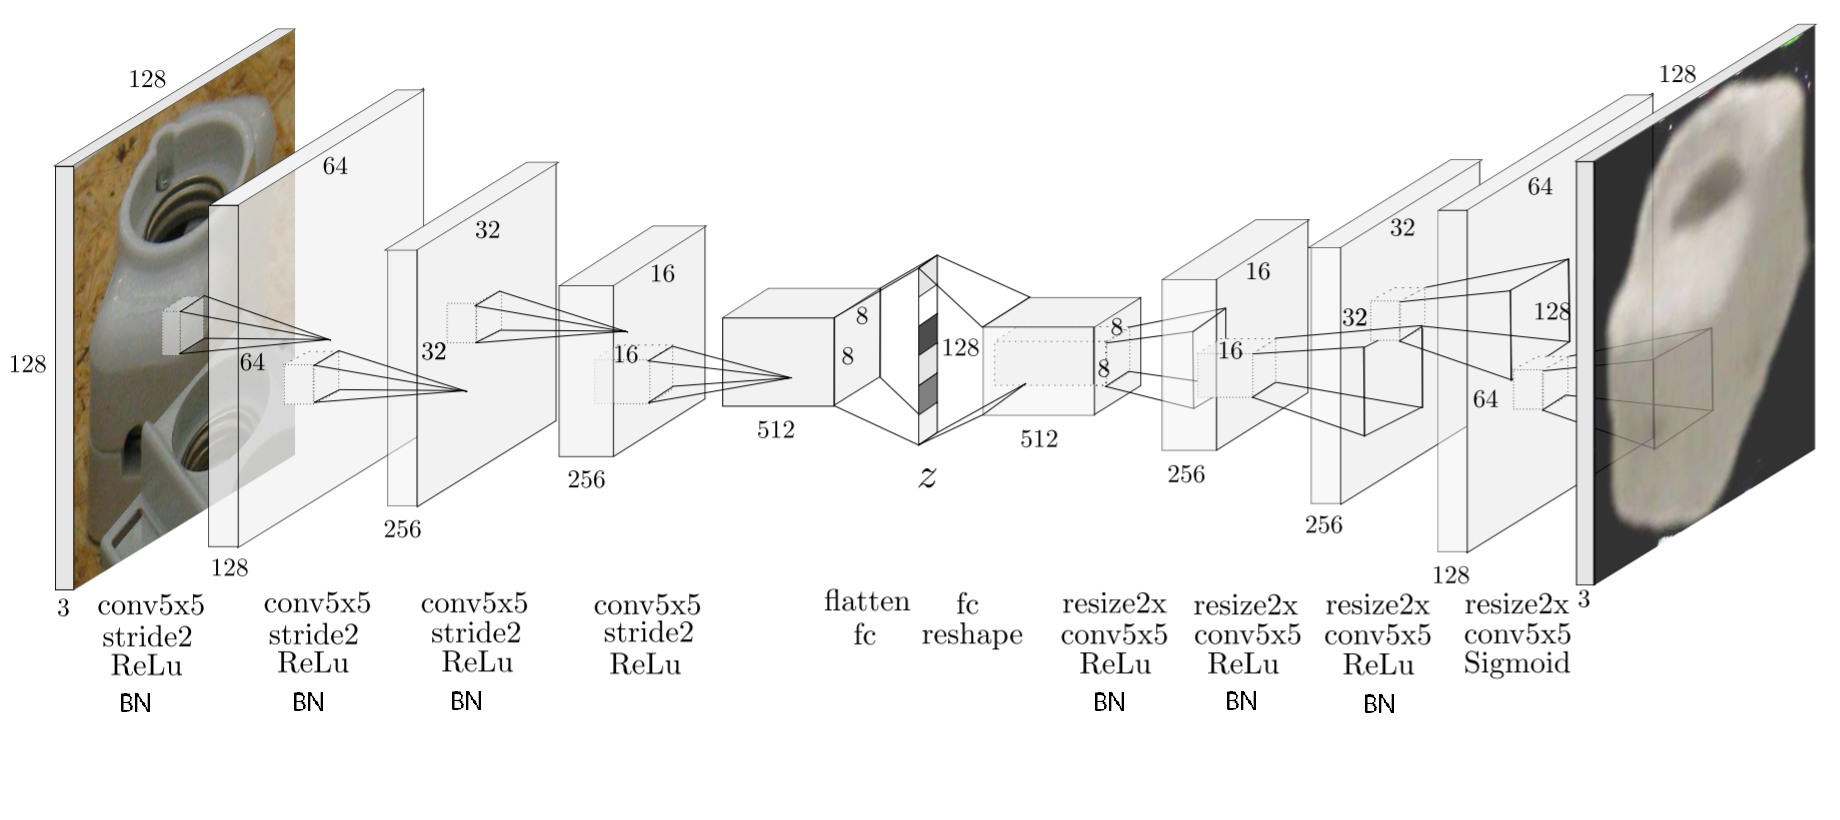
\includegraphics[width=1\textwidth]{newautoencoder}
	\caption[Autoencoder architecture]{\textbf{Autoencoder architecture}}
	\label{fig:newautoencoder}
\end{figure}


After the training, the autoencoder is able to extract the object from real scene crops, while the clarity and the orientation of the decoder reconstruction indicates the encoding quality. 

\section{3D Pose Estimation}
To determine the object orientation, a codebook is firstly created at the offline stage, which contains the latent encodings $z_i \in \mathcal{R}^{128} $ of object views at equidistant viewpoints from a full view-sphere. 
 \\[8pt]
 At test time, the image crops of the considered objects will be resized and forwarded to the encoder network. After encoding, the highest cosine similarity between the test code $z_{test} \in \mathcal{R}^{128}$ and all codes from the codebook will be searched via the nearest neighbor algorithm, and the corresponding rotation matrix will be determined as the object orientation.  
\begin{align}
cos_i = \frac{z_i \, z_{test}}{||z_i||\, ||z_{test}||}
\label{eq:cosineloss} 
\end{align}
\chapter{Evaluation}
\section{Experimental Settings}
\subsubsection{Dataset Generation}

The training set is generated by rendering synthetic views of the object 3D models from uniformly sampled 2562 viewpoints, additionally with 36 in-plane rotations at each viewpoint, together $2562 \times 36 = 92232$ views. 
\\[8pt]
The test set is rendered from randomly sampled 1000 viewpoints on the sphere with random in-plane rotation, i.e. $1000 \times 1 = 1000$ views.
\subsubsection{Dataset Augmentation}
While keeping reconstruction targets clean, following random augmentations are applied to the input images: 
(\romannumeral 1) applying random cropping, translation and resizing; 
(\romannumeral 2) varying image contrast, brightness and color distortions;
(\romannumeral 3) inserting random background images from Lorem Picsum dataset \cite{Picsum}. 


\subsubsection{Training Settings}
During the training of the autoencoder, I used the Adam optimizer with a learning rate of $2 \times 10^{-4}$, a batch size $= 64$..

\newpage
\section{Experimental Results}
\subsection{Visualization of the Training Process}
\begin{figure}[H]
	\subfigure[pitcher base]{
		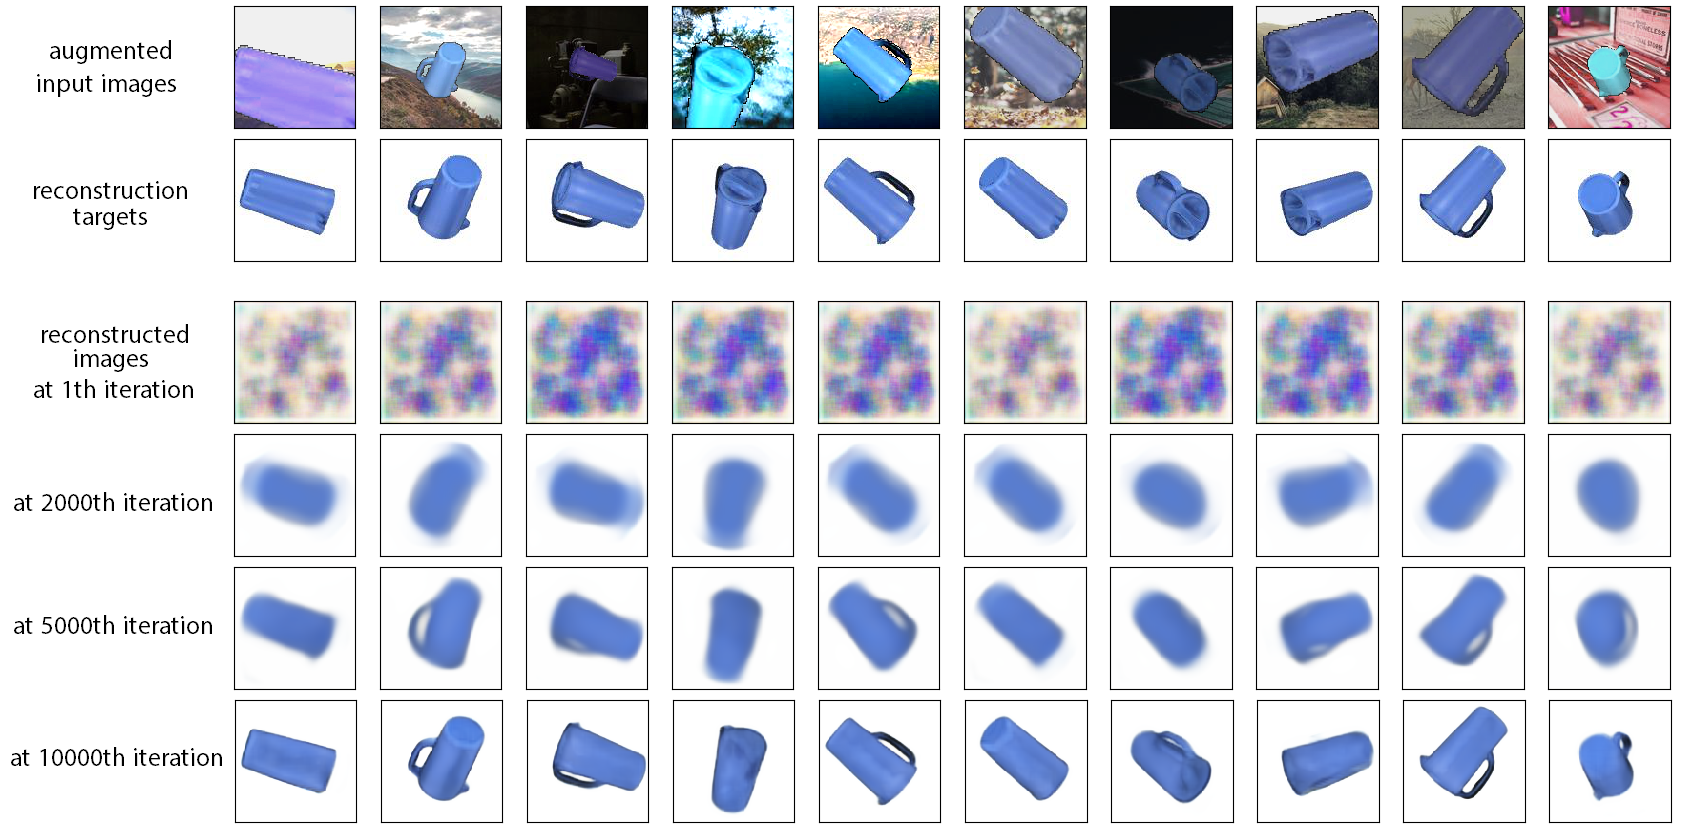
\includegraphics[width=1.05\textwidth]{trainingprocess}
		\label{fig:regular}
	}
	\subfigure[bowl]{
		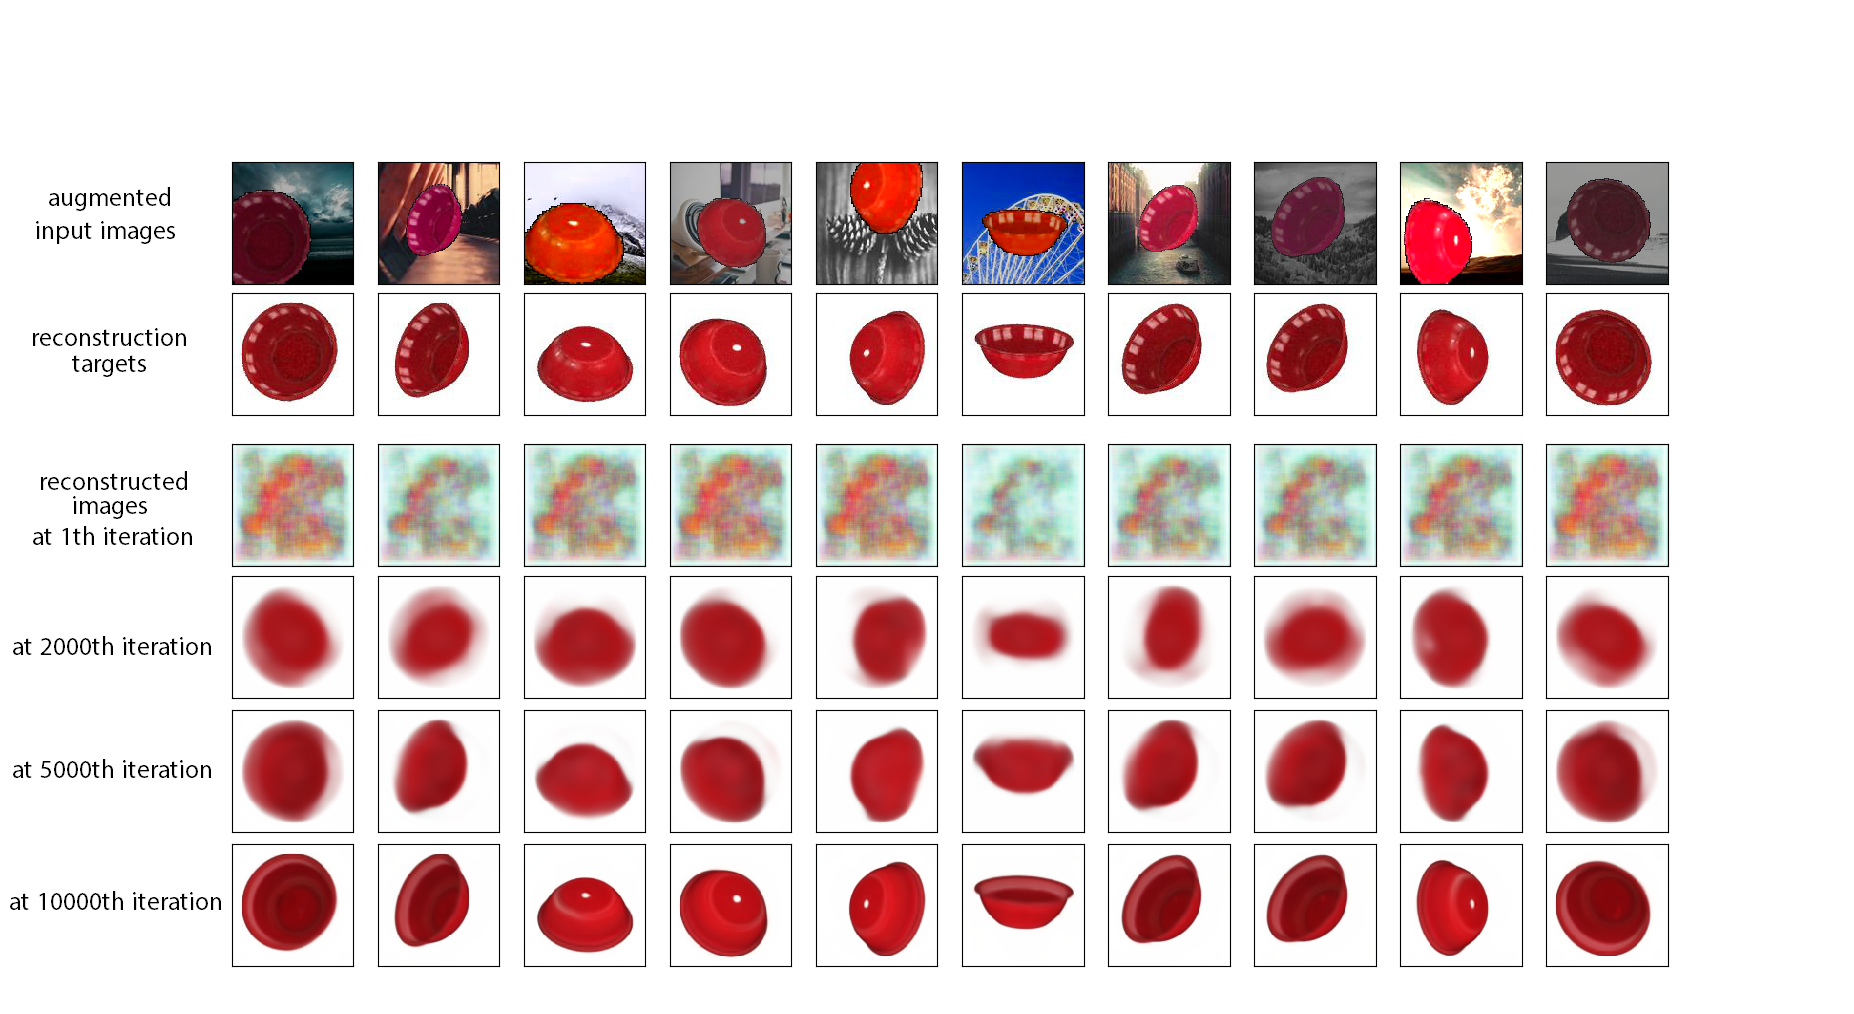
\includegraphics[width=1.15\textwidth]{bowl}
		\label{fig:random}
	}
	\caption[Visualization of the training process]{\textbf{Visualization of the training process}}
	\label{fig:trainingprocess}
\end{figure}


As shown in Fig. \ref{fig:trainingprocess}, the reconstructed images are randomly initialized at the beginning of the training. After around 2000 iterations, the autoencoder is able to extract a vague shape of the object. With the training time going by, the quality of the reconstructed object images increase. After around 10000 iterations, the orientation and the structure of the object can be very good reconstructed.

\subsection{Rotation error}
In order to evaluate the pose estimation results, the rotation error $\theta_{err} $ between the ground truth and the estimated rotation matrix of the object is computed via \ref{eq:error1} and \ref{eq:error2}: 
\begin{align}
	R_{err} = R_1 \cdot R_2^T
	\label{eq:error1} \\	
	\theta_{err} = arccos(\frac{tr(R_{err})-1}{2})
	\label{eq:error2}	
\end{align}


\setlength{\tabcolsep}{20pt}
\renewcommand{\arraystretch}{1.5}
\begin{tabular}{|m{5.5cm} | m{3.0cm}| m{3.0cm}|}

	\hline
	\multicolumn{3}{|c|}{unsymmetrical object (pitcher base)} \\
	\hline
	\diagbox{test set}{training set} &augmented &non-augmented \\
	\hline
	augmented    &0.09796& 2.47153  \\
	\hline
	non-augmented  &0.05773    &0.05556\\
	\hline
	\multicolumn{3}{|c|}{unsymmetrical object (bowl)} \\
	\hline
	\diagbox{test set}{training set} &augmented &non-augmented \\
	\hline
	augmented &0.50277 & 2.18787 \\
	\hline
	 non-augmented &0.12769&  0.22125\\
\hline
\end{tabular}
 \begin{center}
 	Table 3.1: \textbf{Rotation error [radian] between ground truth and estimated pose in different scenarios}
 \end{center}
\vspace{4pt}
The test errors in different scenarios are reported in table 3.1. Based on the testing results, we can come to the following conclusions:\\[8pt] (\romannumeral 1) Because of the pose ambiguities, the rotation error tested on the symmetrical object is larger than unsymmetrical objects. Nevertheless, the orientation of symmetrical objects can still be good extracted as shown in Fig. \ref{fig:trainingprocess}. \\[8pt]
(\romannumeral 2) The autoencoder trained on the non-augmented training set performs very well on the non-augmented testing set. However, it fails to generalize to the augmented dataset.\\[8pt]
(\romannumeral 3) The autoencoder trained on the augmented training set is able to achieve a good performance both on the augmented and on the non-augmented dataset.
%_____Zusammenfassung, Ausblick_________________________________
\chapter{Conclusion}
In this project, I implemented the pose estimation approach proposed in \cite{sundermeyer2018implicit} and tested it in different scenarios. The evaluation result shows that this approach is able to handle the pose ambiguity problem due to the symmetrical structure of objects. Furthermore, it shows a good generalization capability in different environment simulated by dataset augmentation. 
\\[8pt]
However, due to constraints of time and computing power, only the 3D orientation of the object pose is estimated in my project. In the future, the project can be extended to estimate the 6D pose of the object. And stronger augmentation, like occlusions with random object masks may be further applied to the training dataset in order to strengthen the feature extraction capability of the autoencoder against occlusion. 

%%%%%%%%%%%%%%%%%%_Abbildungsverzeichnis %%%%%%%%%%%%%%%%%%%%%%
\cleardoublepage
\addcontentsline{toc}{chapter}{List of Figures}
\listoffigures 	

%%%%%%%%%%%%%%%%%%_Acronyms and Notations %%%%%%%%%%%%%%%%%%%%%%
\cleardoublepage

%%%%%%%%%%%%%%%%%%Literaturverzeichnis %%%%%%%%%%%%%%%%%%%%%%%%
\cleardoublepage
\addcontentsline{toc}{chapter}{Bibliography}
\bibliography{mybib}
\bibliographystyle{alpha}
%%%%%%%%%%%%%%%%%%%%License %%%%%%%%%%%%%%%%%%%%%%%%%%%%%%%%%%%
\cleardoublepage
\chapter*{License}
\markright{LICENSE}
This work is licensed under the Creative Commons Attribution 3.0 Germany
License. To view a copy of this license,
visit \href{http://creativecommons.org/licenses/by/3.0/de/}{http://creativecommons.org} or send a letter
to Creative Commons, 171 Second Street, Suite 300, San
Francisco, California 94105, USA.


\end{document}
